\documentclass[a0paper,landscape, font_size=30pt]{baposter}

\usepackage{lmodern}
\usepackage{amsmath}
\usepackage{fontspec}
\usepackage[utf8]{inputenc}
\usepackage[T1]{fontenc}
\usepackage{colortbl}
\usepackage{arydshln}
\usepackage{booktabs}
\usepackage{forest}
\usepackage{tcolorbox}
\usepackage{multicol}
\usepackage{multirow}
\usepackage{unicode-math}
%\setmainfont{Times New Roman}
\setmainfont{Microsoft Sans Serif}
%\setmainfont{Minion 3 Display}
\setmathfont{STIX Two Math}
\newcommand{\methodname}{PsychoBench}

\newcommand{\compresslist}{
\setlength{\itemsep}{0pt}
\setlength{\parskip}{1pt}
\setlength{\parsep}{0pt}
}


\newenvironment{boenumerate}
{\begin{enumerate}\renewcommand\labelenumi{\textbf\theenumi.}}
{\end{enumerate}}

\definecolor{myblue}{RGB}{144, 155, 255}
\definecolor{myyellow}{RGB}{253, 253, 143}
\definecolor{mypurple}{RGB}{34, 64, 150}
\definecolor{bordercolor}{RGB}{34,64,150}
\definecolor{backgroundcolor}{RGB}{34,64,150}
\definecolor{caltechyellow}{RGB}{255,248,202}
\begin{document}
\begin{poster}
{
grid=false,
headerborder=open, % Adds a border around the header of content boxes
colspacing=1em, % Column spacing
bgColorOne=white, % Background color for the gradient on the left side of the poster
bgColorTwo=white, % Background color for the gradient on the right side of the poster
borderColor=bordercolor, % Border color
headerColorOne=caltechyellow, % Background color for the header in the content boxes (left side)
headerColorTwo=caltechyellow, % Background color for the header in the content boxes (right side)
headerFontColor=mypurple, % Text color for the header text in the content boxes
boxColorOne=white, % Background color of the content boxes
textborder=rounded, %rectangle, % Format of the border around content boxes, can be: none, bars, coils, triangles, rectangle, rounded, roundedsmall, roundedright or faded
eyecatcher=false, % Set to false for ignoring the left logo in the title and move the title left
headerheight=0.11\textheight, % Height of the header
headershape=rounded, % Specify the rounded corner in the content box headers, can be: rectangle, small-rounded, roundedright, roundedleft or rounded
headershade=plain,
%headerfont=\Large\textsf, % Large, bold and sans serif font in the headers of content boxes
%textfont={\setlength{\parindent}{1.5em}}, % Uncomment for paragraph indentation
linewidth=2pt % Width of the border lines around content boxes
}

%
%-----------------------------
%	TITLE AND AUTHOR NAME
%-----------------------------
%
{
\vspace{0.5em}
%\textsf{\color{mypurple}Recent  $\nu$ Cross-Section and FSI Tuning in NOvA }
\color{mypurple}\Huge \hspace*{2em} ProtoDUNE-VD for BSM Searches: Initial Studies and Future Prospects 
}
{
%\sf\vspace{-0.1em} \\
\vspace{-0.6em}
\begin{center}
\textbf{  \hspace{3cm}        Biao Wang$^{1}$,
%on behalf of ProtoDUNE-BSM working group, for the DUNE collaboration
for the DUNE collaboration
}
%on behalf of the ProtoDUNE-BSM Group }% {Biao Wang}$^{(1)}$, Jeremy Wolcott$^{(2)}$ and Hugh R. Gallagher$^{(2)}$
\vspace{-0.1em} \\
\small{  \hspace{3cm} $\bullet$$^{1}$University of Iowa,  IA, USA $\bullet$ Neutrino 2026, Irvine, June 21-26, 2026
}
%\small{Department of Physics and Astronomy, University of Iowa, Iowa City, USA}%{$^{(1)}$~Department of Physics and Astronomy, University of Iowa} \\
%\small{$^{(2)}$~Department of Physics and Astronomy, Tufts University }
\end{center}
}
{
\includegraphics[width=3.5cm,keepaspectratio]{figures/logo.png}}


\headerbox{1. Overview of ProtoDUNE-VD}{name=introduction,span=2,column=0,row=0}{

\begin{itemize}\compresslist
\item Full-scale prototype of the first DUNE Far Detector module, validation of detector R\&D, calibration, reconstruction, and analysis techniques before DUNE operations.
\item Test-beam data provide precise detector-response measurements using known particle species: Electrons, Pions, Kaons and Protons at specific momenta ($0.5$-$8 \text{ GeV/c}$) allow for direct measurement of track-length vs. deposited energy,  charge recombination and $dE/dx$ based PIDs.
\item Unique opportunity to search for BSM physics, and previous studies have characterized both the underlying mechanism and the associated phenomenology~\cite{deGouva_characterizing_2022, Coloma:2023adi}.

\end{itemize}
\vspace{-1.0em}
\begin{center}
    \includegraphics[width=1.0\linewidth]{figures/i03vd}
\end{center}
\vspace{-1.5em}
\begin{itemize}\compresslist
\item Full-streaming: 2 top CRPs + 2 bottom CRPs. Cathode in the middle hanging from the top CRPs.
\item 8 full-streaming Photon Detection modules on the cathode and 8 self-triggering modules on the walls.
\item Future Xenon doping calibration by bottom PMTs.
\end{itemize}
}




\headerbox{2. Opportunities for New Physics}{name=prompt,span=2,column=0,below=introduction}{

\begin{itemize}\compresslist
\item A Heavy Neutral Fermion (HNF) can be produced either via meson decays (e.g., $K^+\to\ell^+N$)~\cite{deGouva_characterizing_2022}, via the Drell-Yan process (e.g., $Z’ \to N \bar{N}$), or through muon bremsstrahlung where a high-energy muon radiates a dark boson that subsequently decays into a fermion pair ($\mu\to \mu \phi, \phi\to N \bar{N}$)~\cite{NA64:2024nwj}.
\end{itemize}

\vspace{-2.5em}

\begin{center}
    \resizebox{1.0\linewidth}{!}{
    \small
    \begin{tabular}{lp{6.6cm}}
    \toprule
    \rowcolor{myblue}
    \multicolumn{2}{l}{\textbf{Key Decay Channels of HNFs:}} \\
    \textsc{$N \to \ell^- K^+/\pi^+$} & Determine the lifetime of HNFs. \\
    \textsc{$N \to \nu X$} & Angular distributions of the boson $X$ (e.g., $\gamma, \pi^0$) probe anisotropy. \\
    \textsc{$N \to \nu \ell^+ \ell^-$} &   Provide rich kinematic final state analysis.\\
    \bottomrule
    \end{tabular}
    }
\end{center}

}

\headerbox{3. CERN SPS T2 Beamline}{name=framework,span=2,column=2}{
\begin{itemize}\compresslist
\item The T2 primary target/wobbling station receives the 400 GeV/c proton beam from the CERN Super Proton Synchrotron (SPS) and uses target, magnet, and collimation elements to produce and select secondary beams. 
\item Generates an intense flux of mesons and muons in a beam-dump environment that can enable studies of Heavy Neutral Fermions (HNFs) and other hidden-sector particles~\cite{Coloma:2023adi},  alongside the ProtoDUNE-VD test-beam program.
\end{itemize}
\vspace{-2.0em}
\begin{center}
    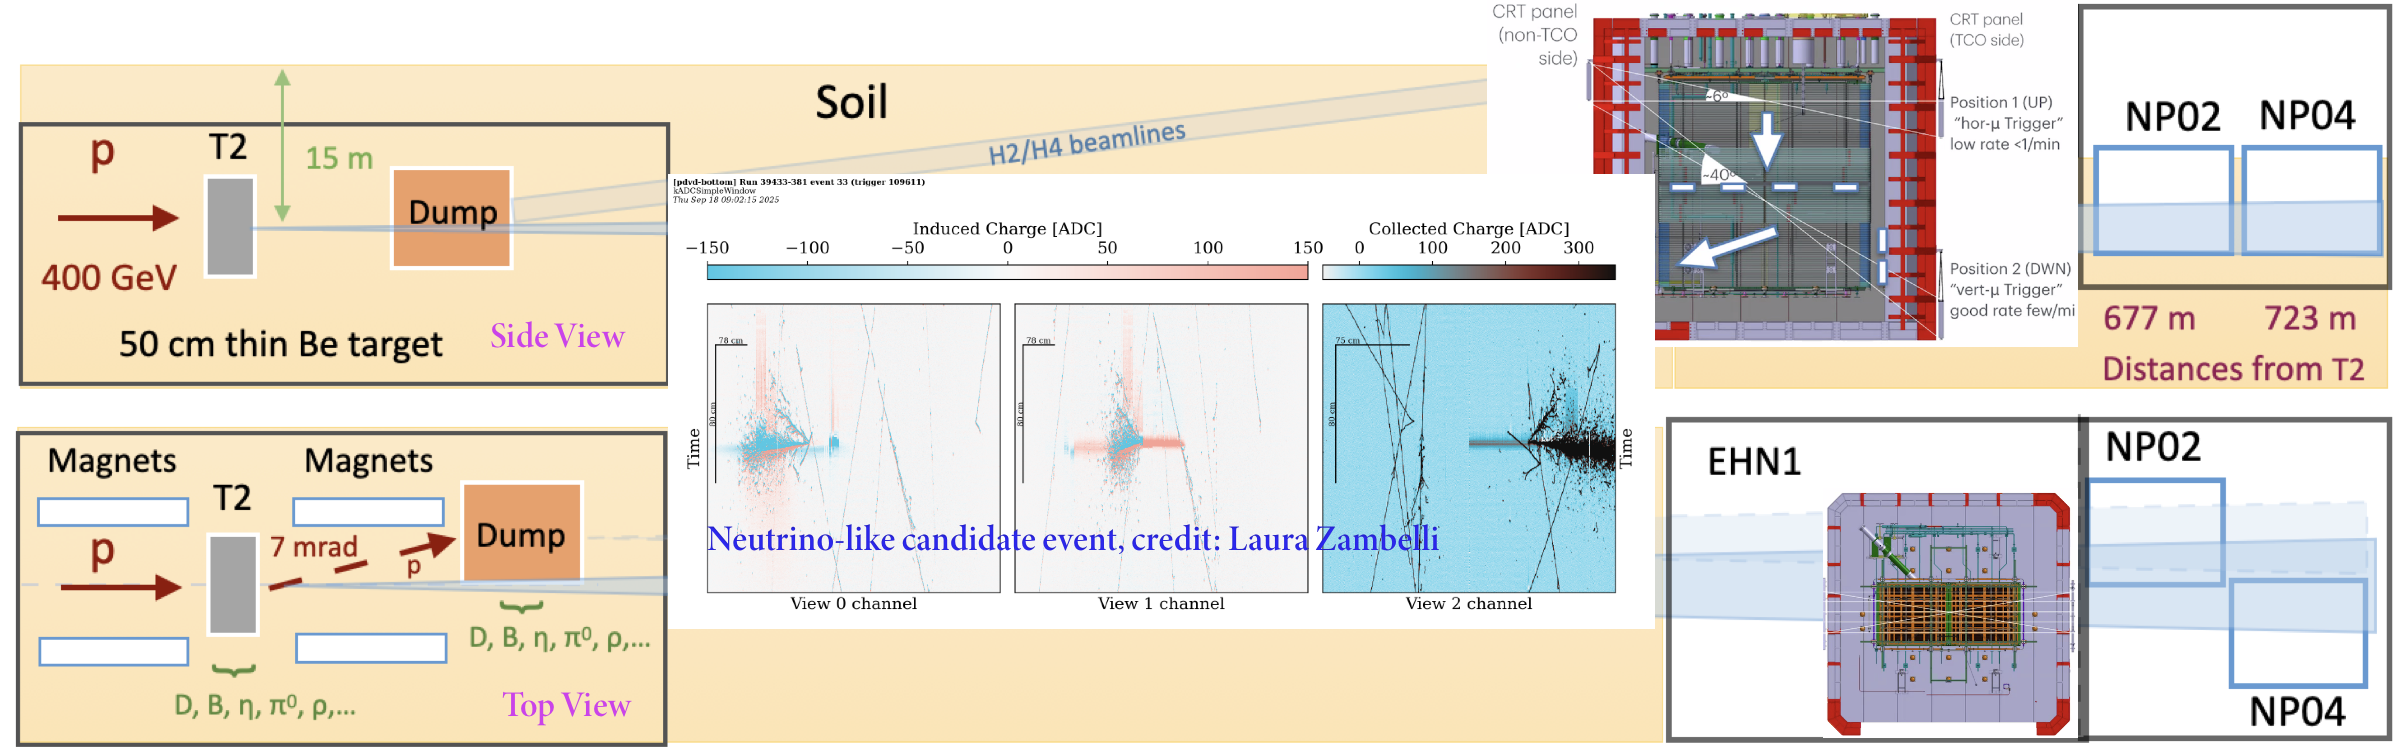
\includegraphics[width=1.0\linewidth]{figures/T2beam.png}
\end{center}
\vspace{-1.1em}

}


\headerbox{4. Trigger Development and Analysis Progress}{name=r1,span=2,column=2,below=framework}{
\begin{itemize}\compresslist
\item ADCSimple trigger selects events with large deposited charge in a short (about 0.2 ms) time window.
\item Optimize the ADC threshold to maximize HNF~($N\to \mu^- \pi^+$) and neutrino signal efficiency while suppressing cosmic backgrounds.
\end{itemize}

\vspace{-2.0em}
\begin{center}
    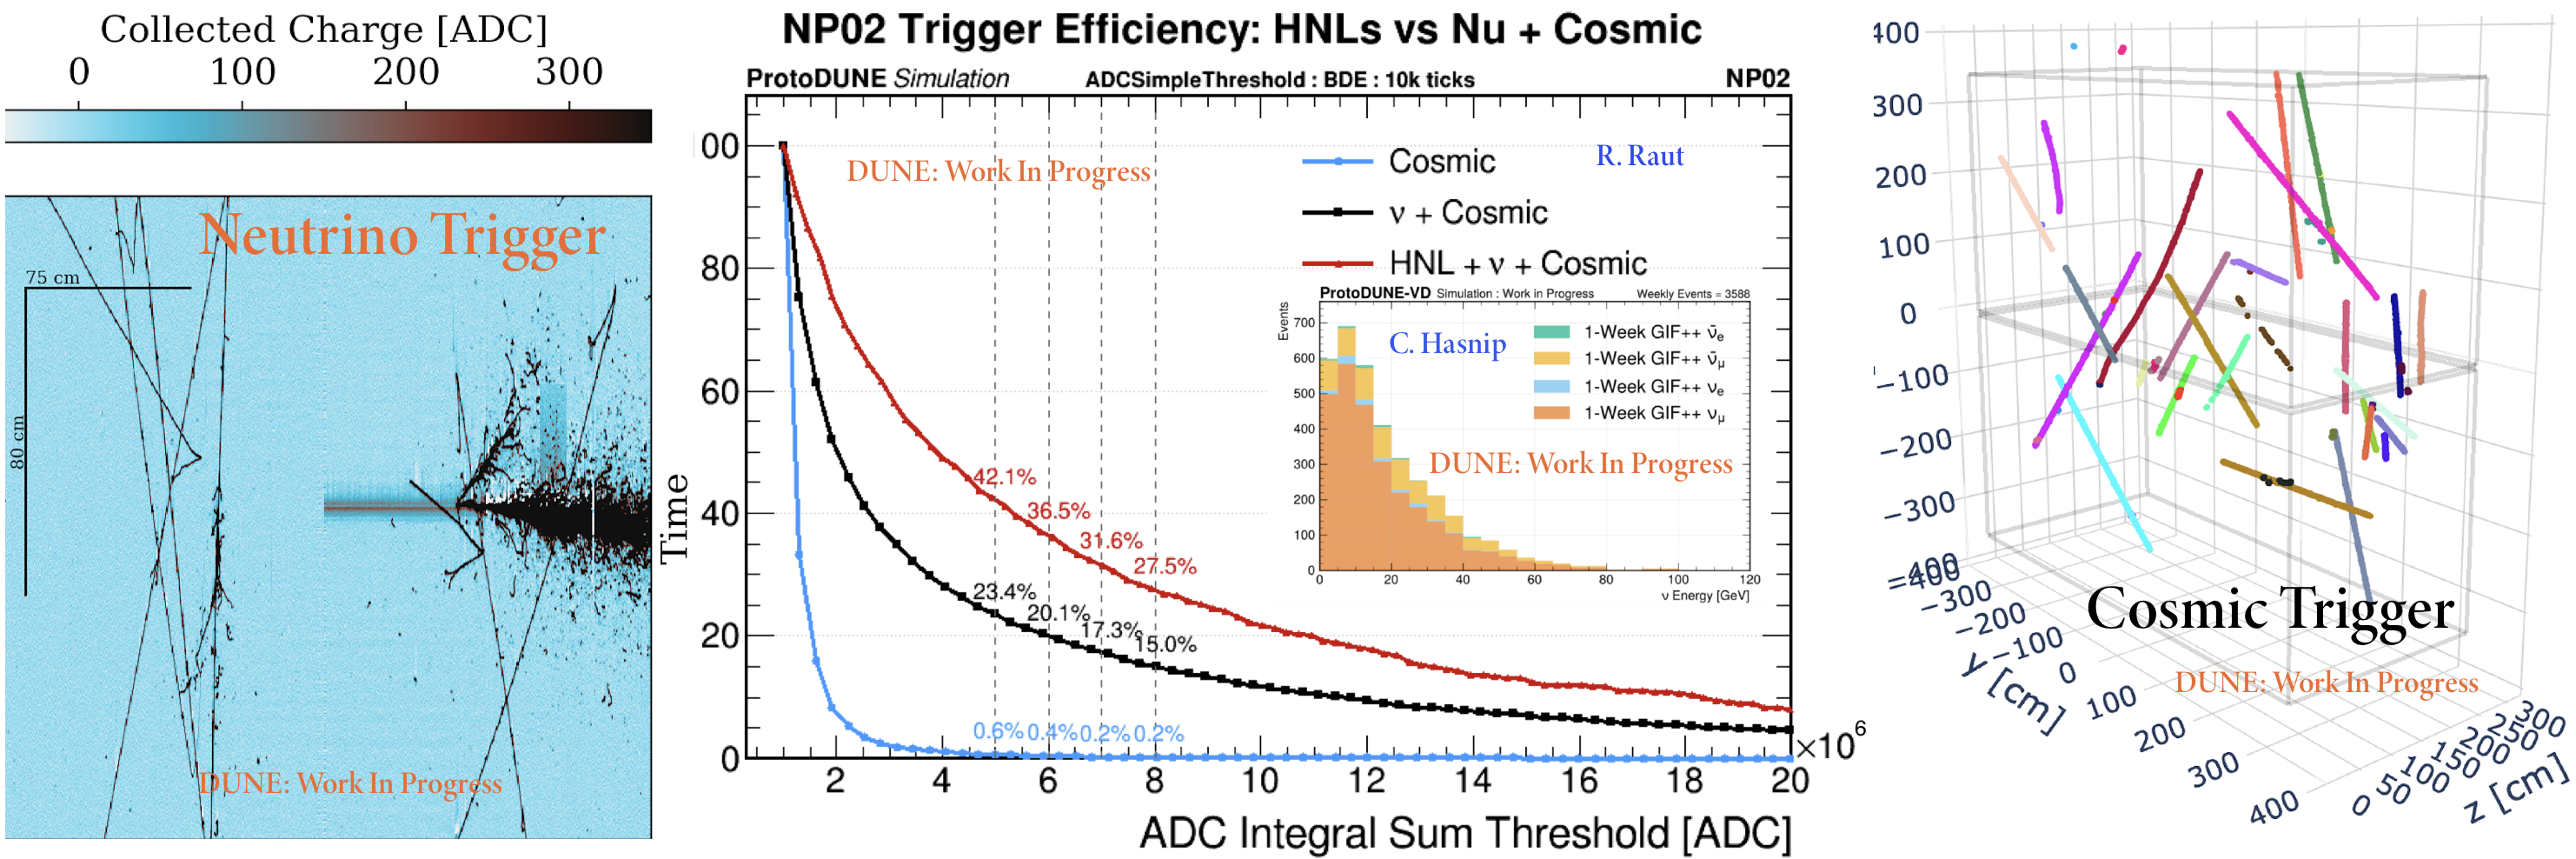
\includegraphics[width=1.0\linewidth]{figures/spine.png}
\end{center}
\vspace{-2.0em}

\begin{itemize}\compresslist
\item Automated reconstruction and event-selection frameworks under development for future DUNE analyses aim to classify high-energy neutrino interactions and potential HNF/BSM signatures, with current iterations showing adaptable performance capabilities~\cite{Drielsma:2021jdv}.

\end{itemize}
}




\headerbox{5. Reference}{name=r3,span=2,column=2,below=r1}{
 \tiny
%\nocite{*} % Insert publications even if they are not cited in the poster
%\renewcommand{\refname}{} % Removes the "References" title
\renewcommand{\section}[2]{\vskip 0.05em} % Get rid of the default "References" section title
\bibliographystyle{unsrt}
\compresslist
\let\oldthebibliography\thebibliography
\let\endoldthebibliography\endthebibliography
\renewenvironment{thebibliography}[1]{%
  \begin{oldthebibliography}{#1}%
    \setlength{\itemsep}{0pt}%
    \setlength{\parsep}{0pt}%
}{%
  \end{oldthebibliography}%
}
\bibliography{poster}

}









\end{poster}
\end{document}
